\documentclass[russian,12pt]{article}
\usepackage{cmap}
\usepackage{mathtext}
\usepackage[russian]{babel}
\usepackage[a4paper, left=2.00cm, right=2.00cm, top=2.00cm, bottom=2.00cm, marginparwidth=1.75cm]{geometry}
\usepackage{amsmath}
\usepackage{amssymb}
\usepackage{fancyhdr}
\usepackage{graphicx}
\usepackage{wrapfig}
\usepackage{array}
\usepackage{nicefrac}

\providecommand{\header}[1]{
    \,
    \begin{center}
        {\Large \textbf{#1}}
    \end{center}
    }
\providecommand{\subheader}[1]{
    \,
    \begin{center}
        {\large \textbf{#1}}
    \end{center}
    }
\providecommand{\headwithsub}[2]{
    \,
    \begin{center}
        {\Large \textbf{#1}} \\ \, \\
        {\large \textbf{#2}}
    \end{center}
    }
\newcommand{\at}{\biggr\rvert}

\title{\textbf{Расчётно-графическая работа №1}}
\author{Студенты 1-го курса бакалавриата КТиУ, СУиР \and Овчинников П.А., Румянцев А.А., Чебаненко Д.А.}
\date{26 июня 2023 г.}
\pagestyle{fancy}
\fancyhf{}
\fancyhead[L]{Математический анализ (весна'23)}
\fancyfoot[C]{\thepage}
\begin{document}
\maketitle
\header{Определение $\delta$-функции Дирака}
\textbf{Дельта-функция} --- распределение, введённое физиком Полем Дираком, с помощью которого можно записать точечное воздействие или показать плотность физических величин, сосредоточенных или приложенных в одной точке. Формально эта обобщённая функция представляет собой линейный функционал, который отображает функцию только в её нулевом значении. Также известен символ $\delta$ Кронекера, который по сути является дискретным аналогом символа $\delta$ Дирака и часто применяется в линейной алгебре.
\begin{figure}[!h]
    \centering
    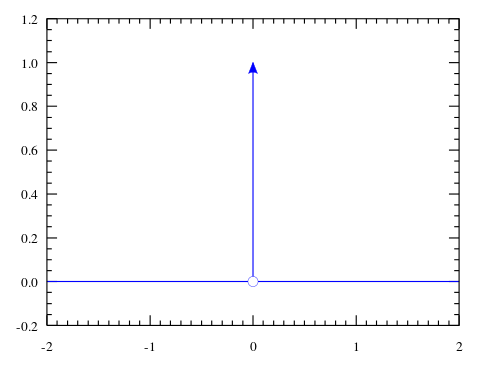
\includegraphics[width=0.5\textwidth]{graph}
    \begin{center}{\footnotesize Рис. 1: Одномерный график дельта-функции}\end{center}
\end{figure} \\
Определим дельта-функцию через финитные бесконечно дифференцируемые функции.
\subheader{Финитные бесконечно дифференцируемые и обобщённые функции}
Функция, определённая во всём пространстве $R^m$ и равная нулю во всех достаточно удалённых точках $R^m$, т.е. в точках, удовлетворяющих условию $\left\lvert x\right\rvert > M$, где $M$ --- некоторое положительное число, называется обычно финитной функцией в $R^m$. Класс \textbf{финитных бесконечно дифференцируемых} в $R^m$ функций (т.е. \textbf{основных функций}) обозначается через $C^{\infty}_0(R^m)$ (его ещё обозначают как $D$). Число $M$ для различных функций $u(x)$ этого класса может быть, естественно, различным. Рассмотрим функцию $u(x)$, суммируемую по всему пространству $R^m$, т.е. $u(x)$ из $L_1(R^m)$. Обозначим через $u_{(M)}(x)$ функцию, совпадающую с $u(x)$ в шаре $\left\lvert x\right\rvert < M$ и равную нулю в остальных точках $R^m$. Так как $u \in L_1(R^m)$, то:
$$\int\left\lvert u(x)-u_{(M)}(x)\right\rvert dx = \int\limits_{\left\lvert x\right\rvert > M}\left\lvert u(x)\right\rvert dx \rightarrow 0 \text{ при } M \rightarrow \infty.$$ \\ \, \\
Формально \textbf{обобщённая функция} или, другими словами, распределение $f(\varphi)$ определяется как линейный непрерывный функционал над тем или иным векторным пространством основных функций.

\subheader{Определение дельта-функции через финитные бесконечно дифференцируемые}
Пусть $\varphi(x)$ --- финитная бесконечно дифференцируемая функция и $x \in \mathbb{R}$. Тогда $\varphi(x) \in C^{\infty}_0$. Дельта-функцией Дирака называется линейная непрерывная обобщённая функция, действующая на функции $\varphi(x)$ по правилу $\hat{\delta}\varphi = \varphi(0)$ или, по другому говоря:
$$\int\limits_{-\infty}^{+\infty}\delta(x)\varphi(x)dx = \varphi(0).$$
Действие дельта-функции согласно такому простому правилу расширяется на все функции $\varphi(x)$, определённые и непрерывные в некоторой окрестности нуля. Поскольку результат действия дельта-функции определяется только значением $\varphi(x)$ в нуле, то:
\begin{align*}
    \int\limits_{a}^{b}\delta(x)\varphi(x)dx = \varphi(0)\qquad & \qquad \int\limits_{a}^{b}\delta(x)\varphi(x)dx = 0, \\
    a<0<b\qquad\qquad\;\;                                       & \;\;\qquad\qquad0 \notin [a, b]
\end{align*}
Символ $\delta(x)$ не является функцией в обычном смысле слова --- дельта-функция, как и всякая обобщённая функция, является оператором и задаётся исключительно способом её действия на основные функции $\varphi(x)$. 
$\delta$-функция может выражаться через пределы:
$$\delta(x) = \lim_{\alpha \rightarrow \infty}\frac{\sin\alpha x}{\pi x} \qquad \delta(x) = \frac{1}{\sqrt{\pi}}\lim_{\alpha \rightarrow 0}\alpha\text{e}^{\nicefrac{-x^2}{\alpha^2}} \qquad \delta(x) = -\lim_{\alpha \rightarrow 0}\frac{\text{e}^{\nicefrac{x}{\alpha}}}{\alpha(\text{e}^{\nicefrac{x}{\alpha}} + 1)^2}$$

\headwithsub{Свойства $\delta$-функции}{Фильтрующее свойство функции}
Рассмотрим интеграл $\int\delta(x-x_0)\varphi(x)dx, \quad \varphi(x) \in D$ и сделаем в нём замену переменной $t = x - x_0$:
$$\int\delta(x-x_0)\varphi(x)dx = \int\delta(t)\varphi(t+x_0)dt = \varphi(x_0).$$
Таким образом $\int\delta(x-x_0)\varphi(x)dx = \varphi(x_0)$.

\subheader{Чётность $\delta$-функции}
Рассмотрим интеграл $\int\delta(-x)\varphi(x)dx = \varphi(0), \quad \varphi(x) \in D$ и вновь сделаем замену $t = -x$:
$$\int\delta(-x)\varphi(x)dx = - \int\delta(t)\varphi(-t)dt = \int\delta(x)\varphi(-x)dx = \varphi(0).$$
Таким образом $\int\delta(-x)\varphi(x)dx = \varphi(0) = \int\delta(x)\varphi(-x)dx \;\Rightarrow\; \delta(-x)=\delta(x)$.
\pagebreak

\subheader{Первообразная $\delta$-функции. Функция Хевисайда}
Ступенчатая функция Хевисайда является обобщённой первообразной дельта-функции. Её уравнение довольно незамысловато:
$$\theta(x) = \begin{cases}
    0, \quad x < 0, \\
    1, \quad x > 0.
\end{cases}$$
Покажем взаимосвязь этих функций:
$$\int\limits_{-\infty}^{+\infty}\theta'(x)\varphi(x)dx = \theta(x)\varphi(x)|^{+\infty}_{-\infty} - \int\limits_{-\infty}^{+\infty}\theta(x)\varphi'(x)dx = - \int\limits_{0}^{+\infty}\varphi'(x)dx = $$
$$= -\varphi(x)|^{+\infty}_{0} = \varphi(0) = \int\limits_{-\infty}^{+\infty}\delta(x)\varphi(x)dx.$$
Это и означает, что $\theta'(x) = \delta(x)$, т.е. дельта-функция является обобщённой производной функции Хевисайда.
\begin{figure}[!h]
    \centering
    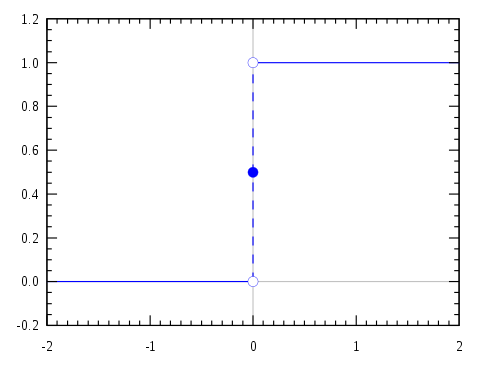
\includegraphics[width=0.5\textwidth]{heavyside}
    \begin{center}{\footnotesize Рис. 2: График первообразной функции Хевисайда}\end{center}
\end{figure}

\header{Приложения}
Дельта-функция крайне полезна и удобна для описания различных физических явлений, в которых приходится иметь дело с точечными объектами и источниками
\subheader{Плотность распределения тепла}
Пусть функция $f(x, t)$ описывает плотность распределения источников тепла на прямой, т. е. определяет, какое количество тепла выделяется в точке $x$ в момент времени t. Такие свойства
\begin{enumerate}
    \item Если в точке $x_0$ непрерывный источник тепла мощности $Q$, то функцию $f(x, t)$ запишем в виде $Q\delta(x-x_0)$.
    \item Если в точке $x_1$ в момент времени $t_1$ мгновенно выделяется количество тепла $Q$, тогда $f(x, t)=Q\delta(x-x_1)\delta(t-t_1)$.
    \item Пусть в точке $x_1$ находится непрерывно-действующий источник мощности $Q_1$, в точке $x_2$ - источник, который выделяет в момент времени $t_2$ количества тепла, равное $Q_2$, тогда $f(x, t)=Q_1\delta(x-x_1)+Q_2\delta(x-x_2)\delta(t-t_2)$.
\end{enumerate}

\subheader{Плотность тока}
Плотность тока, который создает при своем движении единственный электрон, можно записать в виде: $\vec{j}=\rho\vec{v}$, где $\vec{v}$ - скорость электрона, а $\rho= e\delta(\vec{r} - \vec{r}_0)$ - плотность его заряда.
$$\int\limits_{\mathbb{R}_n}\delta(x)dx = \lim_{\varepsilon \rightarrow 0} \int\limits_{\mathbb{R}_n}\delta_\varepsilon(x)dx = 1$$
Физический смысл этого интеграла --- распределение плотности (единичного заряда, единичной массы и пр.) в виде импульса с носителем в начале координат.\\ \, \\
\textit{\textbf{Nota bene.} Более строго функцию Дирака следовало бы определить как ядро интегрального преобразования.}

\subheader{Теория вероятности}
Дельта-функция часто применяется для представления дискретного распределения и вычисления плотности вероятности в статистике.
Плотность вероятности дискретного распределения, состоящего из точек $x = \left\{x_1, x_2, \dots, x_n\right\}$ с вероятностями $p_1, p_2, \dots, p_n$, может быть записана в виде:
$$P(x) = \sum\limits_{i=1}^n p_i\delta(x-x_i).$$

\end{document}